\newpage

\section{Rotación}

Para realizar la rotación, es necesario saber la posición en el instante anterior de la pelota, y la posición en el instante actual, para así obtener el vector con la dirección (por simplicidad lo llamaré ``v''). También es necesario obtener ``v'' normalizado para realizar otros cálculos (lo llamaré ``w'').

\bigskip

Una vez obtenido ``w'' y haciendo uso del vector normal de la superficie obtenido en la intersección de rayos, se hace el producto vectorial para así obtener el eje de giro.

\bigskip

Por último, para saber cuantos grados debe rotar la pelota, es necesario calcular la distancia de ``v'', de forma que así se obtenga la distancia que ha recorrido. Después, se debe utilizar la fórmula de la longitud del arco de circunferencia, poniendo como incógnita el ángulo. Se debe hacer así porque hay que convertir la distancia recta en distancia circular, para calcular los ángulos. 

\bigskip

La fórmula de la longitud de la circunferencia, cuya incógnita es el ángulo, es: $\alpha = \frac{180 \cdot L}{\pi \cdot r} $, donde L es la longitud recorrida y r el radio de la pelota.

\bigskip

El código para realizar esto es:

% codigo [firstline=300,lastline=500]
\lstinputlisting[language=MaxScript,firstline=40,lastline=65]{../eje_MerloTrujilloAndres_AO_P6.ms}

Cabe destacar que esta función no se debe ejecutar en el primer instante, al necesitar tener el valor de posición de la pelota guía en el instante anterior, por lo que hay que esperar al segundo instante para que empiece a funcionar.

\bigskip
\newpage

A continuación muestro algunas imágenes de la rotación:

% dos o tres fotos en los mismos instantes que antes de la traslacion
\begin{figure}[H]
    \centering 
	\begin{subfigure}[t]{0.48\textwidth}
	    \centering
	    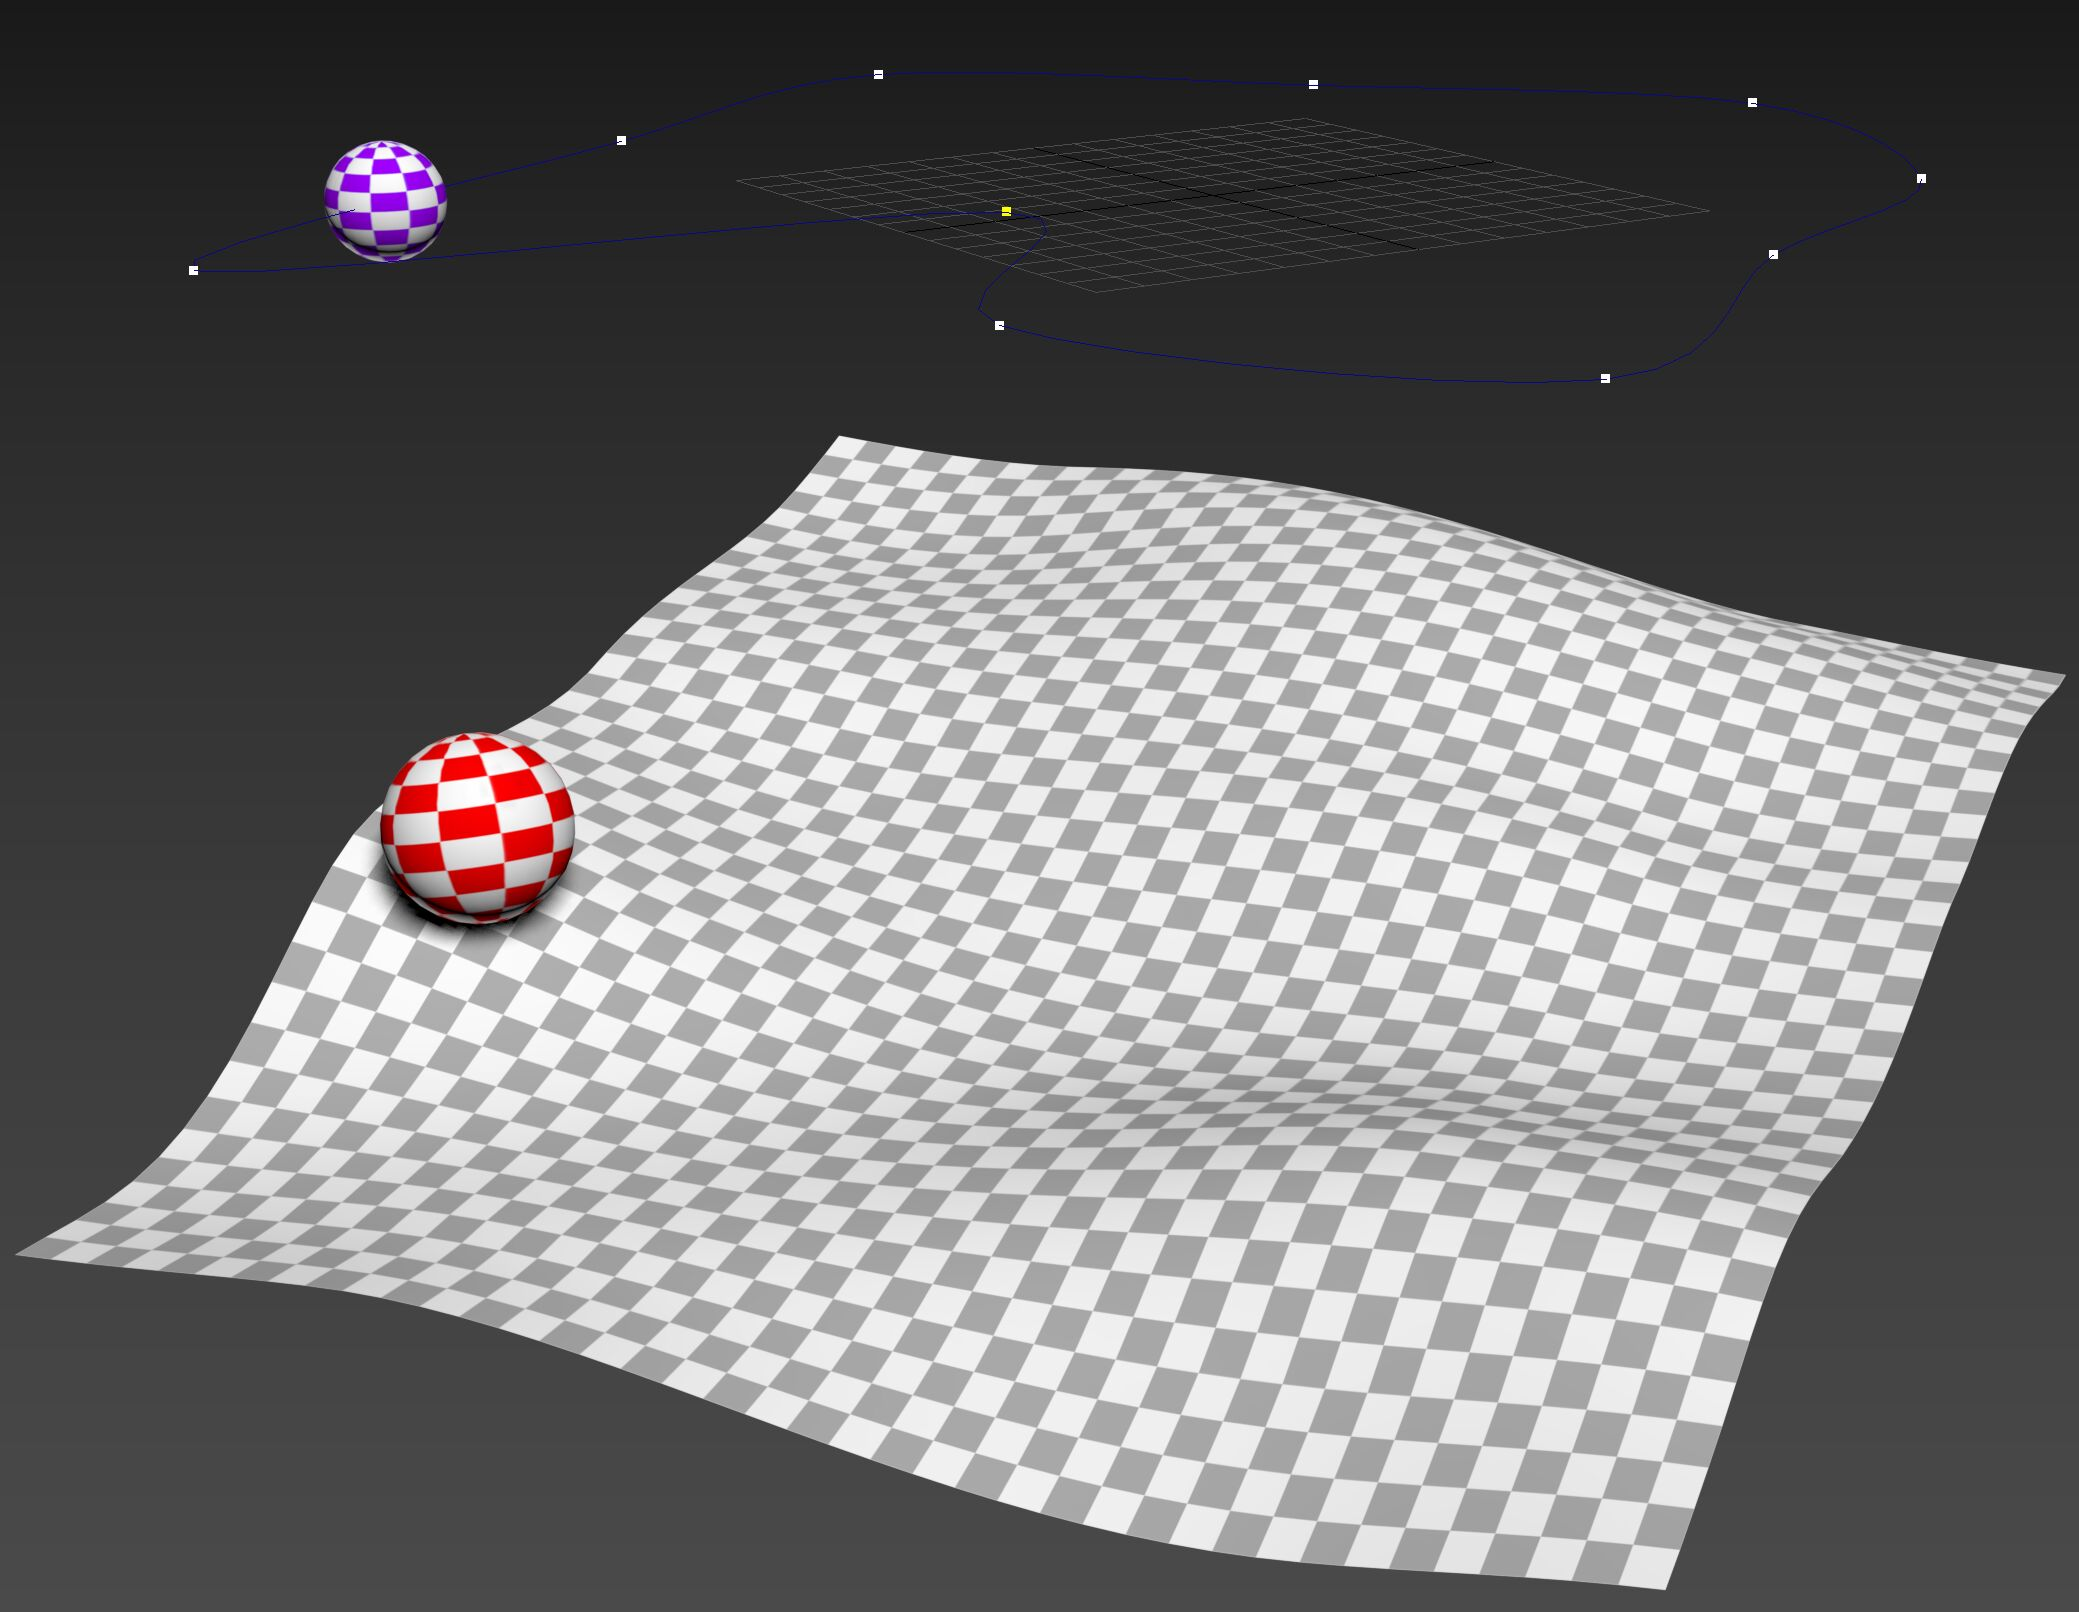
\includegraphics[width=\textwidth]{imagenes/rotacion/100.jpg}
        \caption{Pelotas en el instante 100.}
    \end{subfigure}
    \hfill 
	\begin{subfigure}[t]{0.48\textwidth}
	    \centering
	    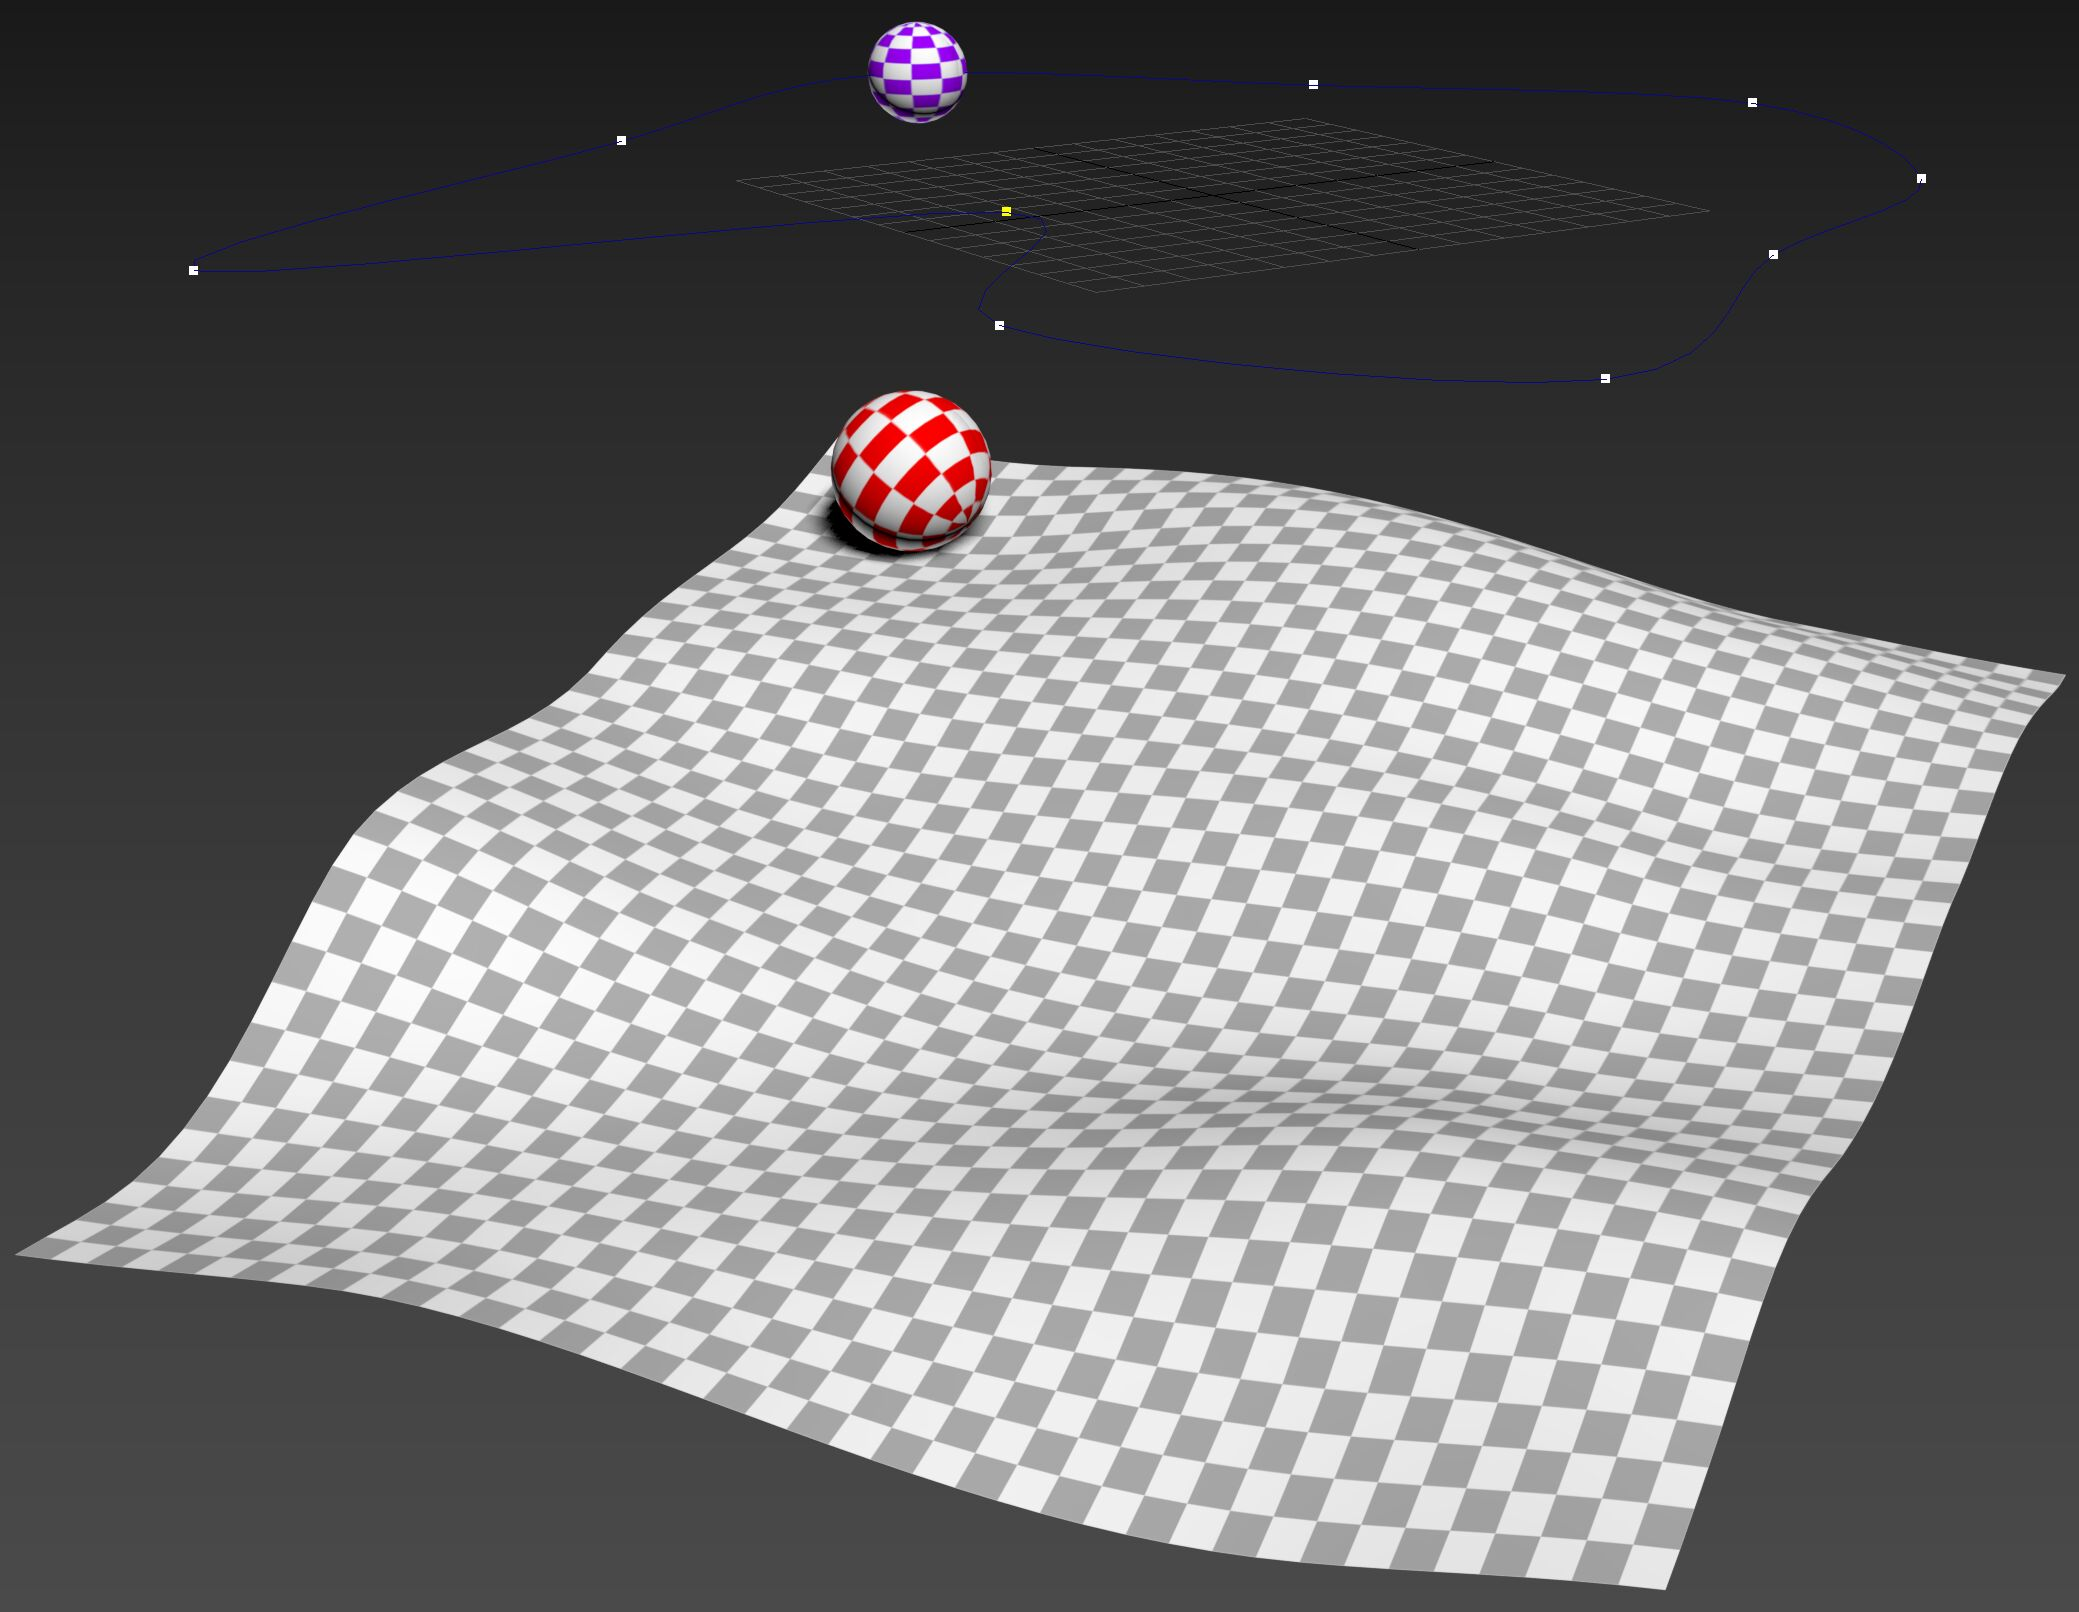
\includegraphics[width=\textwidth]{imagenes/rotacion/185.jpg}
        \caption{Pelotas en el instante 185.}
    \end{subfigure}    
    \par\bigskip
	\begin{subfigure}[t]{0.48\textwidth}
	    \centering
	    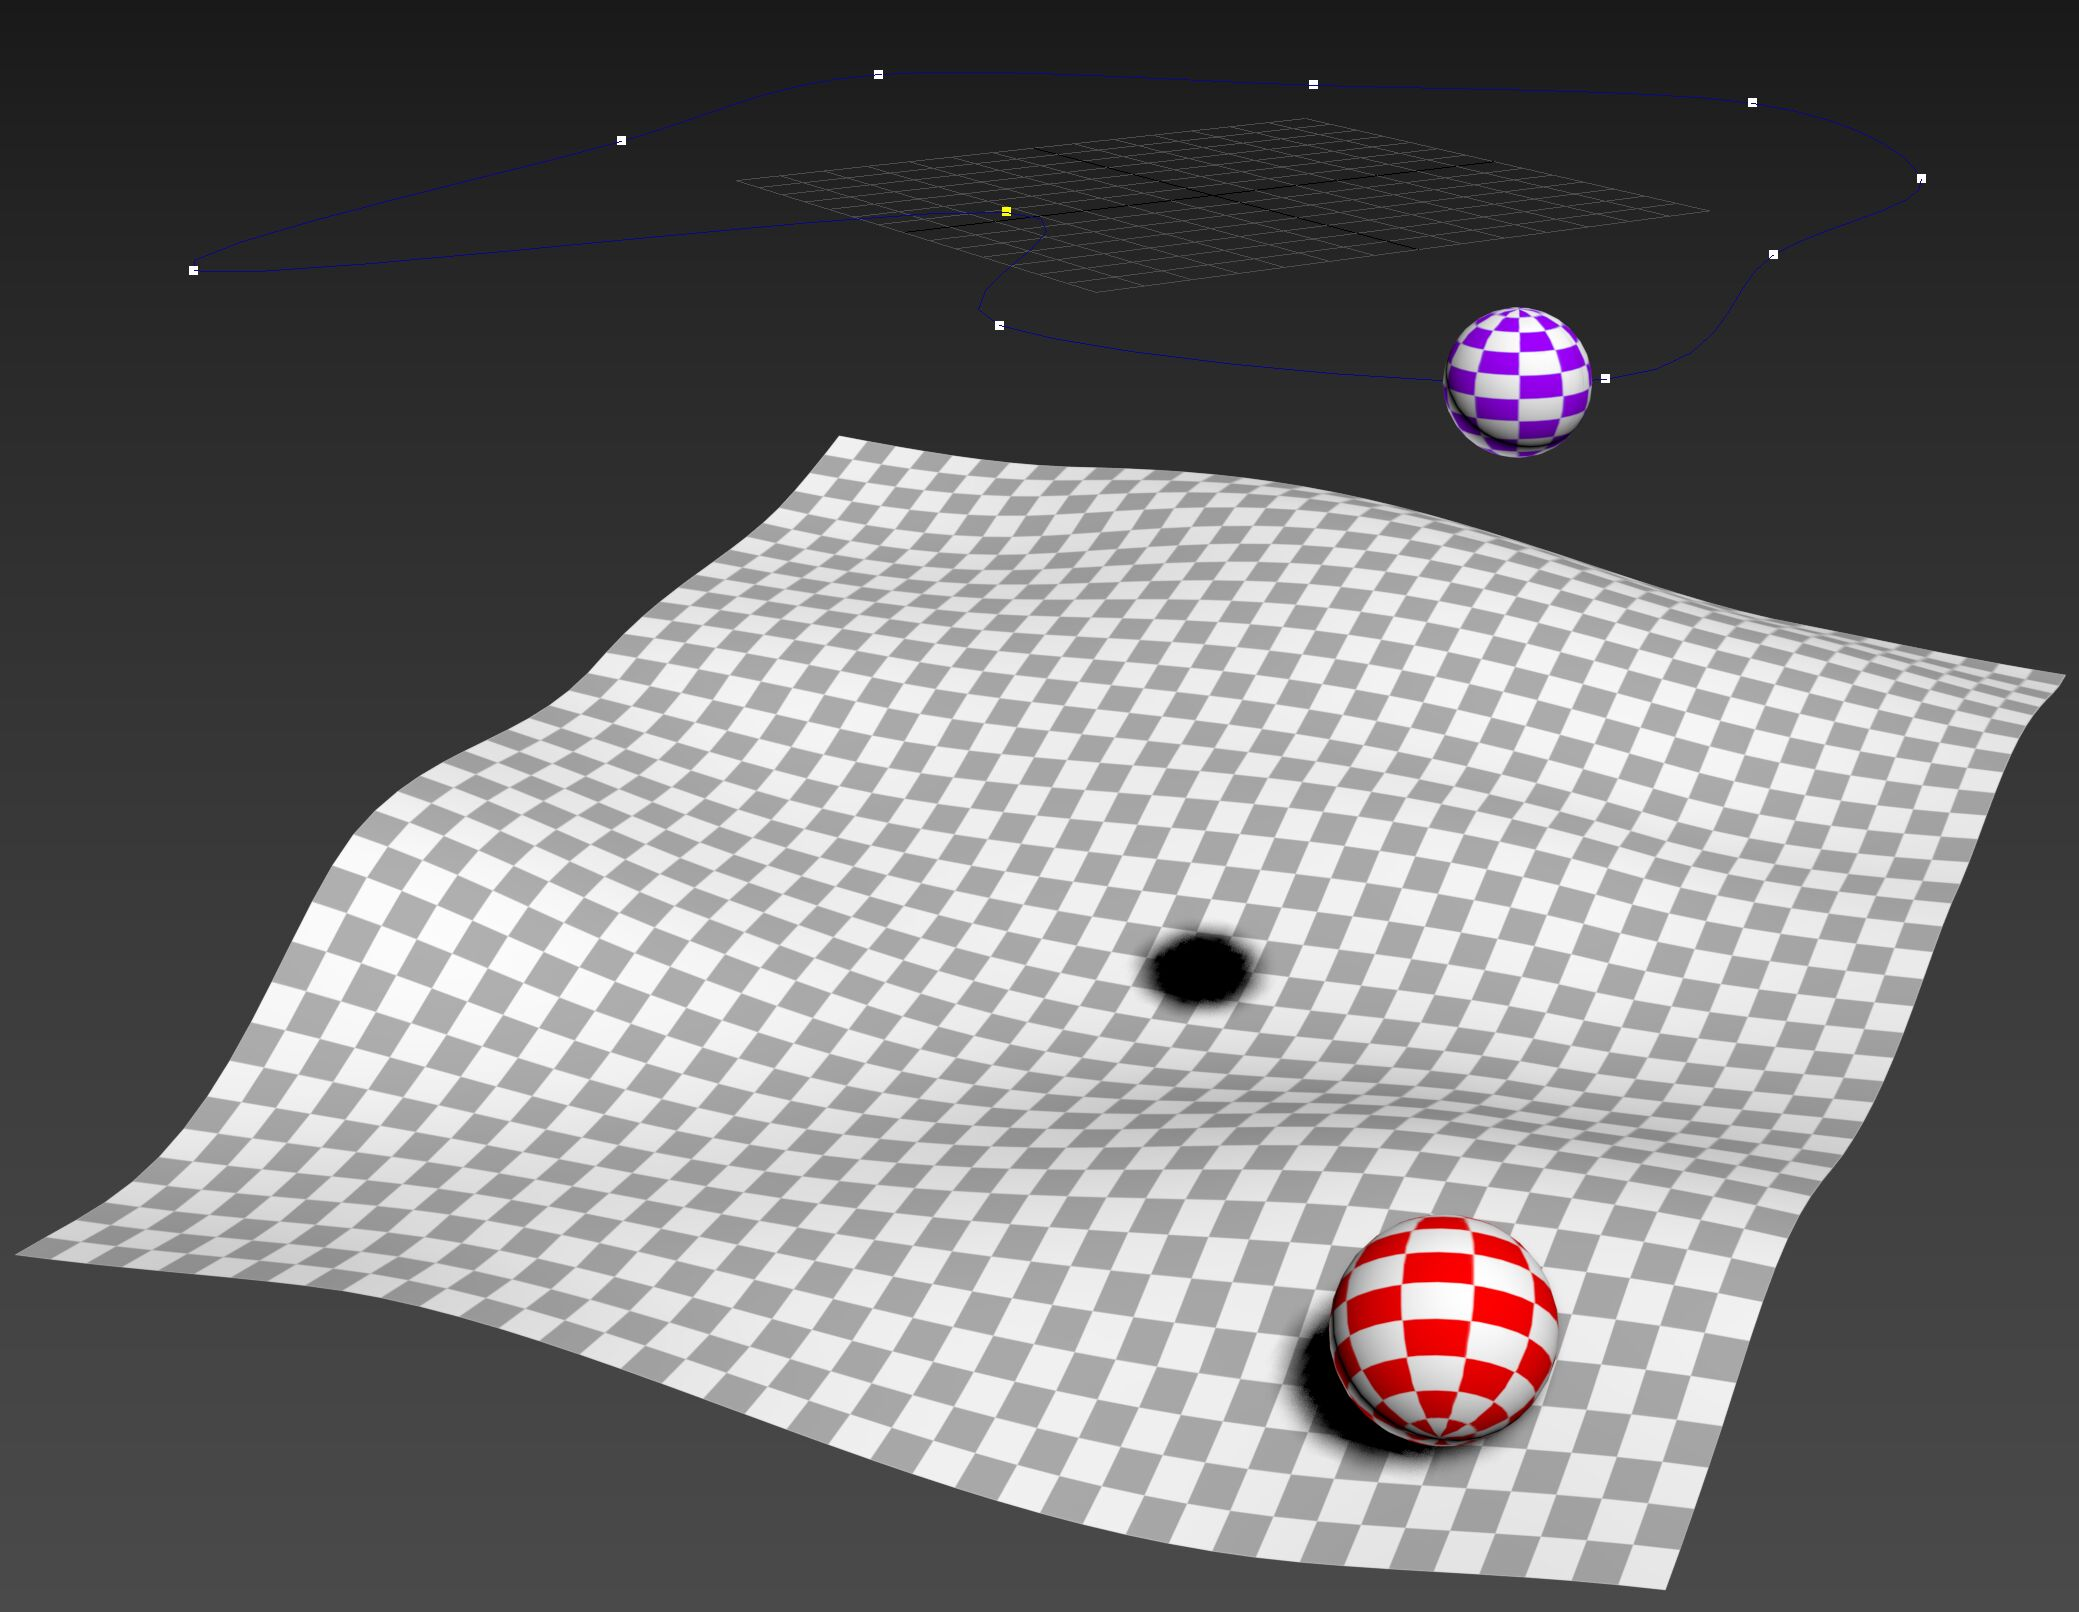
\includegraphics[width=\textwidth]{imagenes/rotacion/410.jpg}
        \caption{Pelotas en el instante 410.}
    \end{subfigure}        
    \caption{Visualización de algunos instantes de la animación final.}
\end{figure}